\section{Clase 1}
\subsection{Generación de variables aleatorias por transformación inversa}

\subsubsection{De una densidad a una función de distribución}

Muchos métodos de simulación parten de un generador de números uniformes
independientes, $U\sim\mathcal{U}(0,1)$. La transformación inversa convierte
esos valores uniformes en observaciones con una distribución objetivo.

Una función $f$ es una densidad de probabilidad si $f(x)\geq0$ y su integral
sobre todo el soporte vale uno. La función de distribución acumulada (FDA) es
\[
    F(x)=\Pr(X\leq x)=\int_{-\infty}^{x} f(t)\,dt.
\]
La FDA es no decreciente y toma valores entre cero y uno. Si se parte de una
función no negativa $\tilde f$ que no está normalizada, primero se calcula
$c=\int_{-\infty}^{\infty}\tilde f(t)\,dt$ y se usa la densidad
$f(x)=\tilde f(x)/c$.

Cuando $F$ es continua y estrictamente creciente, tiene inversa. En ese caso,
la regla de generación es
\[
    U\sim\mathcal{U}(0,1),\qquad X=F^{-1}(U).
\]
En efecto, para cualquier $x$,
\[
    \Pr(X\leq x)
    =\Pr\bigl(F^{-1}(U)\leq x\bigr)
    =\Pr\bigl(U\leq F(x)\bigr)
    =F(x),
\]
por lo que $X$ tiene precisamente la distribución deseada. Si $F$ no es
estrictamente creciente, se utiliza la inversa generalizada
\[
    F^{-1}(u)=\inf\{x\in\mathbb{R}:F(x)\geq u\}.
\]
Esta definición también sirve para distribuciones discretas.

\subsubsection{Algoritmo}

Para generar $N$ observaciones independientes:
\begin{enumerate}
    \item Obtener $N$ valores independientes $U_1,\ldots,U_N$ de una uniforme
    en $(0,1)$.
    \item Calcular $X_i=F^{-1}(U_i)$ para cada $i=1,\ldots,N$.
    \item Usar $X_1,\ldots,X_N$ como la muestra de la distribución objetivo.
\end{enumerate}
El paso esencial es encontrar o evaluar la inversa de la FDA\@. A continuación
se muestran ejemplos donde esa operación puede hacerse explícitamente.

\subsubsection{Ejemplo 1: una densidad creciente en $[0,1]$}

Sea
\[
    f(x)=\begin{cases}2x,&0\leq x\leq1,\\0,&\text{en otro caso.}\end{cases}
\]
La integral de $f$ entre cero y uno es uno. En el intervalo de interés, su FDA
y su inversa son
\[
    F(x)=\int_0^x 2t\,dt=x^2,
    \qquad F^{-1}(u)=\sqrt{u}.
\]
Por tanto, basta generar $U\sim\mathcal{U}(0,1)$ y tomar $X=\sqrt U$. Por
ejemplo, si $U=0.36$, entonces $X=0.6$. La transformación favorece valores
cercanos a uno, como corresponde a una densidad $f(x)$ que crece en ese
sentido. La figura compara la densidad con la FDA, que acumula el área bajo
ella.

\begin{figure}[htbp]
\centering
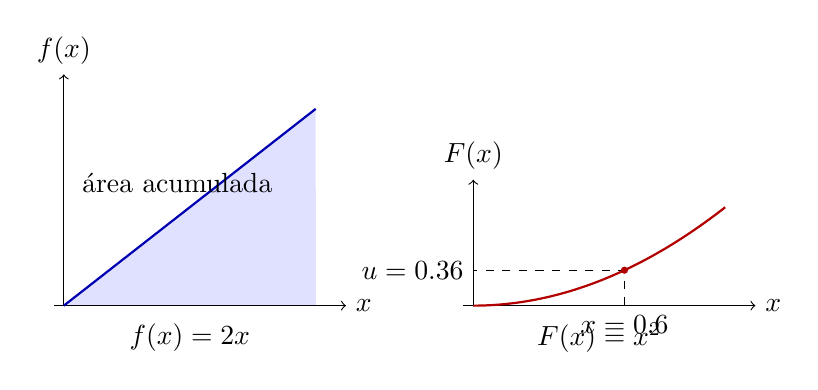
\begin{tikzpicture}[x=3.2cm,y=1.25cm]
  \begin{scope}
    \fill[blue!12] (0,0) -- plot[domain=0:1,samples=50] (\x,{2*\x}) -- (1,0) -- cycle;
    \draw[->] (-0.04,0) -- (1.12,0) node[right] {$x$};
    \draw[->] (0,0) -- (0,2.35) node[above] {$f(x)$};
    \draw[thick,blue!70!black,domain=0:1,samples=50] plot (\x,{2*\x});
    \node[below] at (0.5,-0.08) {$f(x)=2x$};
    \node at (0.45,1.25) {área acumulada};
  \end{scope}
  \begin{scope}[xshift=5.2cm]
    \draw[->] (-0.04,0) -- (1.12,0) node[right] {$x$};
    \draw[->] (0,0) -- (0,1.28) node[above] {$F(x)$};
    \draw[thick,red!70!black,domain=0:1,samples=50] plot (\x,{\x*\x});
    \draw[dashed] (0.6,0) -- (0.6,0.36) -- (0,0.36);
    \fill[red!70!black] (0.6,0.36) circle (1.3pt);
    \node[below] at (0.5,-0.08) {$F(x)=x^2$};
    \node[left] at (0,0.36) {$u=0.36$};
    \node[below] at (0.6,0) {$x=0.6$};
  \end{scope}
\end{tikzpicture}
\caption{La FDA $F(x)=x^2$ integra la densidad $f(x)=2x$. El nivel $u=0.36$ corresponde al cuantil $x=F^{-1}(u)=0.6$.}\label{fig:clase1-densidad-fda}
\end{figure}

\subsubsection{Ejemplo 2: distribución exponencial}

La distribución exponencial de tasa $\lambda>0$ tiene densidad
\[
    f(x)=\begin{cases}\lambda e^{-\lambda x},&x\geq0,\\0,&x<0.\end{cases}
\]
Al integrar se obtiene $F(x)=1-e^{-\lambda x}$ para $x\geq0$. Despejando $x$
en $u=F(x)$,
\[
    u=1-e^{-\lambda x}
    \quad\Longrightarrow\quad
    F^{-1}(u)=-\frac{1}{\lambda}\ln(1-u).
\]
Así, si $U\sim\mathcal{U}(0,1)$, la variable
\[
    X=-\frac{1}{\lambda}\ln(1-U)
\]
sigue la distribución exponencial de tasa $\lambda$. Como $1-U$ también es
uniforme en $(0,1)$, se usa a menudo la forma equivalente
$X=-\ln(U)/\lambda$. Por ejemplo, con $\lambda=1$ y $U=0.7$,
$X=-\ln(0.3)\approx1.204$.

En la primera figura se ve cómo una altura uniforme $u$ selecciona un punto
sobre la función de distribución acumulada. La segunda muestra la misma
operación usando la curva inversa.

\begin{figure}[htbp]
\centering
\begin{tikzpicture}[x=2.1cm,y=3.0cm]
  \draw[->] (-0.08,0) -- (3.35,0) node[right] {$x$};
  \draw[->] (0,0) -- (0,1.12) node[above] {$F(x)$};
  \draw[thick,blue!70!black,domain=0:3,samples=80] plot (\x,{1-exp(-\x)});
  \draw[dashed] (0,0.7) -- (1.204,0.7) -- (1.204,0);
  \fill[blue!70!black] (1.204,0.7) circle (1.5pt);
  \node[left] at (0,0.7) {$U=0.7$};
  \node[below] at (1.204,0) {$X=-\ln(0.3)\approx1.204$};
  \node[blue!70!black,anchor=west] at (2.1,0.82) {$F(x)=1-e^{-x}$};
\end{tikzpicture}
\caption{Para una exponencial de tasa $\lambda=1$, el valor uniforme $U=0.7$ se traza hasta la FDA y determina el cuantil $X=F^{-1}(0.7)$.}\label{fig:clase1-mapeo-fda}
\end{figure}
\begin{figure}[htbp]
\centering
\begin{tikzpicture}[x=6cm,y=1.8cm]
  \draw[->] (-0.03,0) -- (1.04,0) node[right] {$u$};
  \draw[->] (0,0) -- (0,3.45) node[above] {$F^{-1}(u)$};
  \draw[thick,red!70!black,domain=0.01:0.96,samples=90] plot (\x,{-ln(1-\x)});
  \draw[dashed] (0.7,0) -- (0.7,1.204) -- (0,1.204);
  \fill[red!70!black] (0.7,1.204) circle (1.5pt);
  \node[below] at (0.7,0) {$0.7$};
  \node[left] at (0,1.204) {$1.204$};
  \node[anchor=west] at (0.12,3.1) {$F^{-1}(u)=-\ln(1-u)$};
\end{tikzpicture}
\caption{La FDA inversa transforma cualquier $U$ uniforme en un valor exponencial. Aquí se muestra de nuevo $U=0.7$.}\label{fig:clase1-inversa}
\end{figure}

\subsubsection{Distribuciones discretas e inversas no explícitas}

Para una variable discreta con valores $x_1<x_2<\cdots<x_k$ y probabilidades
$p_1,\ldots,p_k$, se acumulan las probabilidades y se devuelve el primer $x_j$
cuya suma acumulada es al menos $U$. Por ejemplo, si
\[
    \Pr(X=0)=0.2,\qquad \Pr(X=1)=0.5,\qquad \Pr(X=2)=0.3,
\]
la regla es
\[
    X=\begin{cases}
        0,&0<U\leq0.2,\\
        1,&0.2<U\leq0.7,\\
        2,&0.7<U<1.
    \end{cases}
\]
La longitud de cada intervalo es igual a la probabilidad del valor que le
corresponde.

No siempre se puede despejar $F^{-1}$ mediante una fórmula elemental. Si se
puede evaluar $F(x)$, se puede hallar $x$ resolviendo $F(x)=U$ numéricamente;
por ejemplo, mediante búsqueda por bisección cuando $F$ es monótona. La
transformación inversa es especialmente sencilla cuando la FDA y su inversa
son fáciles de calcular.

\subsubsection{Resumen}

La transformación inversa convierte una muestra uniforme en una muestra con
la FDA deseada: se calcula $F$ integrando la densidad normalizada, se genera
$U\sim\mathcal{U}(0,1)$ y se obtiene $X=F^{-1}(U)$. Para una FDA discreta o no
estrictamente creciente se usa la inversa generalizada.